\documentclass{article}
\usepackage{graphicx}
\usepackage{geometry}
 \geometry{
 a4paper,
 total={170mm,257mm},
 left=3mm,
 top=18mm,
 }

\title{Tutorial 11: An Introduction to SQL Server Analysis Services and Data Warehousing}
\author{
	Jin, Ziyang\\
	\texttt{\# 34893140}\\
	\texttt{f4a0b}
	\and
	Kim, Joon Hyung\\
	\texttt{\# 35183128}\\
	\texttt{l1m8}
}

\begin{document}
	\maketitle

\section{Deliverable 1}

User would like to use \textbf{drill down} to see the contribution to the total sales for a specific kind of product, or a specific category of products. An example question that drill down can answer is ``In my total sales, how much does Washington Apple Juice contribute to the sales?"\\
\\
User would like to use \textbf{roll up} to see the summarized statistics, such as total sales and total expenses. An example question that roll up can answer is ``Given the salary of each employee, how much does the company pay in total for all the salaries?"

\section{Deliverable 2}

Drill down on the drink products and find \textit{Washington Apple Juice}

\begin{enumerate}
	\item The grand total of all daily unit sales is \textbf{426}.
	\item \begin{enumerate}
			\item \textbf{Sunday} has the highest number of sales for that product.
			\begin{itemize}
				\item Monday 71
				\item Tuesday 50
				\item Wednesday 51
				\item Thursday 48
				\item Friday 51
				\item Saturday 58
				\item Sunday 97
			\end{itemize}
			\item The sales are \textbf{not} evenly distributed. Sunday and Monday have significantly higher sales than the rest of the week. Sunday and Monday are the days when people usually do grocery so the sales are higher.
		\end{enumerate}
	\item A business want to track the total number of unit sales on a particular day to determine how many sales they made on that day. For example, if the business has a promotion event on that particular day, the business would like to measure how effective the promotion is by counting the total sales on that day.
	\item A business want to identify outliers because they don't want to make business decisions imprecisely on these outliers. For example, Washington Apple Juice is very unpopular in a retail shop. One day, some tourists who happen to travel to the city and go into the shop and buys all the Washington Apple Juice -- this outlier data should be excluded because the Washington Apple Juice is unpopular for the shop's daily customers so the shop should not increase the stock.
\end{enumerate}

\section{Deliverable 3}

The Data Cube from Step 4 is a roll up of the MDX query results because it summarizes unit sales across all categories into a total number. 71551 + 557863 + 147346 = 776760. It is a higher level of aggregation of the MDX query result.\\
\\
\noindent The MDX query results are a drill-down of the total unit sales in the Data Cube from Step 4. It drills down the total unit sales to three categories --- drink, food, and non-consumable. So it is a lower level aggregation.

\section{Deliverable 4}

My user id is: \textbf{f4a0b} \\
\\
\noindent 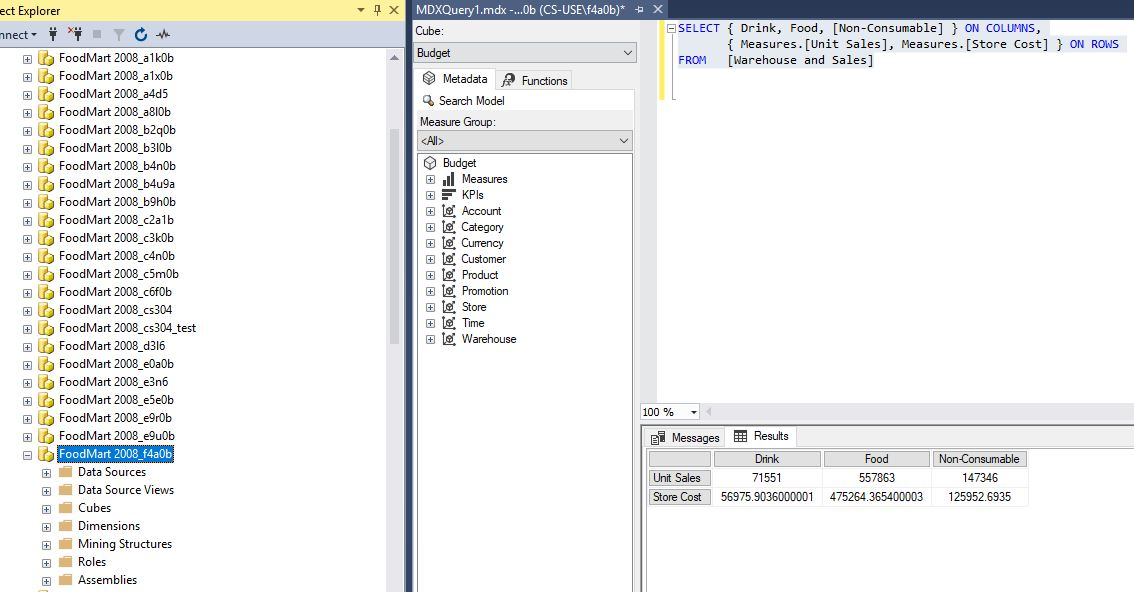
\includegraphics[scale=0.68]{deliverable4.jpg}

\section{Deliverable 5}

\texttt{a) Query Unit Sales and Store Cost of "Drink".}\\

\noindent 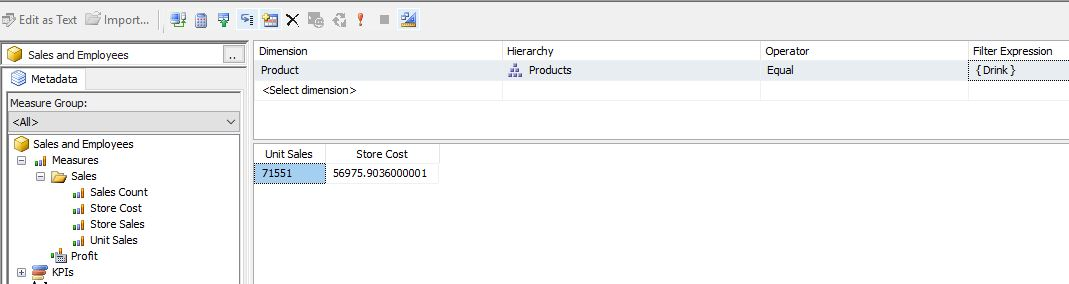
\includegraphics[scale=0.72]{deliverable5_1.jpg}\\
\\
\noindent \texttt{b) Query Unit Sales and Store Cost of "Food".}\\

\noindent 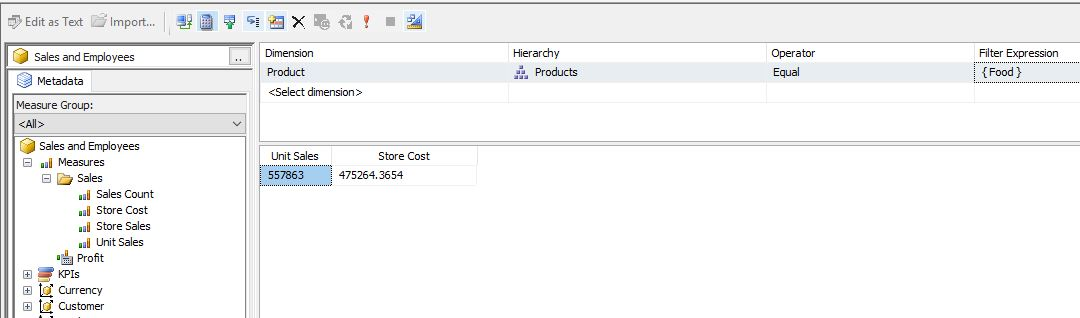
\includegraphics[scale=0.71]{deliverable5_2.jpg}\\
\\
\noindent \texttt{c) Query Unit Sales and Store Cost of "Non-Consumable".}\\

\noindent 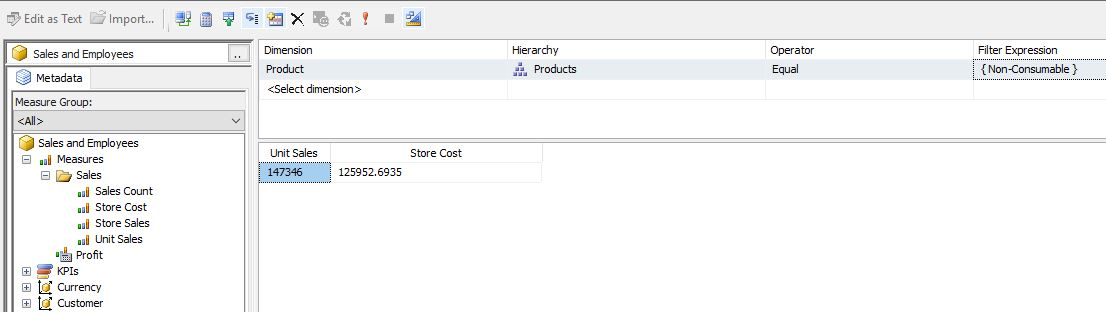
\includegraphics[scale=0.7]{deliverable5_3.jpg}

\section{Deliverable 6}

Choose (a) -- creating and running an MDX query

\begin{verbatim}
SELECT { [Bachelor Degree], [Graduate Degree], [High School Degree] } ON COLUMNS,
       { Measures.[Employee Count], Measures.[Overtime Count] } ON ROWS
FROM   [HR]
\end{verbatim}

\noindent 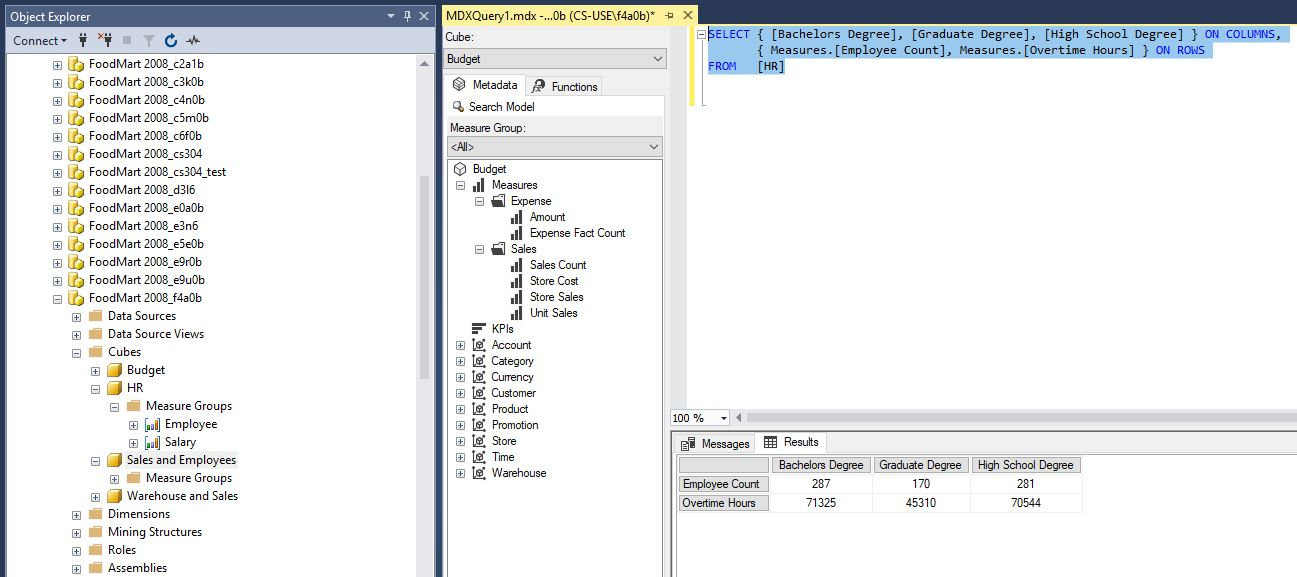
\includegraphics[scale=0.6]{deliverable6.jpg}\\
\\
\noindent \textbf{Explanation:}\\
\\
This query result answers the question``How does education level of employees affect their overtime hours". We can see that 287 Bachelor employees work 71325 overtime hours -- on average 249 hours/employee; 170 Graduate employees work 45310 overtime hours -- on average 267 hours/employee; 281 High School employees work 70544 overtime hours -- on average 251 hours/employee. So employees with Graduate degrees tend to work overtime more often.

\section{Deliverable 7}

I drilled down on the sales of soda drinks categorized by different brands and different quarters of year 1997.\\
\\
\noindent 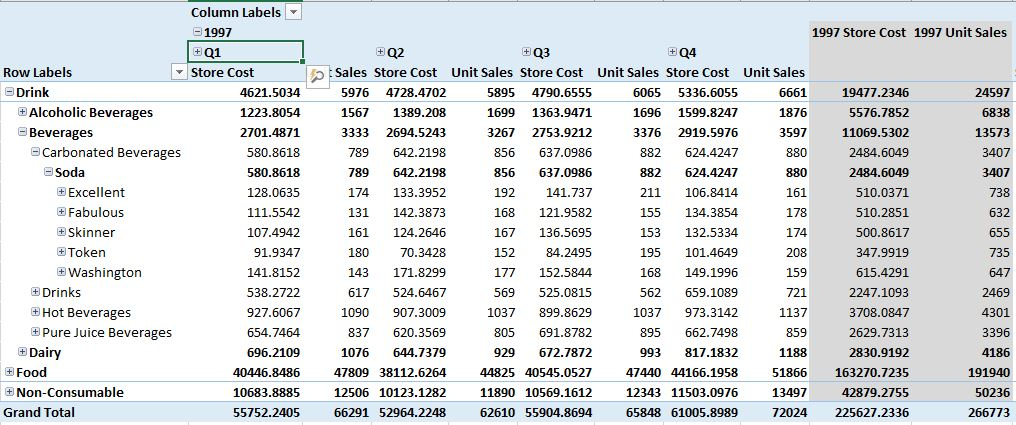
\includegraphics[scale=0.61]{deliverable7.jpg}


\end{document}
